\documentclass[12pt,a4paper,twoside]{article}
%\documentclass[12pt,a4paper,twocolumn,twoside]{article}
\usepackage[utf8]{inputenc}
\usepackage[english]{babel}
\usepackage{amsmath}
\usepackage{amsfonts}
\usepackage{amssymb}
\usepackage{graphicx}
\usepackage{parcolumns}
\usepackage[left=2.5cm,right=2.5cm,top=2.5cm,bottom=2.5cm]{geometry}
\usepackage[final]{pdfpages} %serve per aggiungere altre pagine pdf al file
\usepackage{siunitx}
\usepackage{booktabs}	% better tables
\usepackage{multirow}

\usepackage{caption}		% to use subfigure
\usepackage{subcaption}
\usepackage{sidecap}


\usepackage{svg}			% to include svgs

\author{Davide Bazzanella}
\title{Improving phase-matching of FWM with temperature}

\makeatletter
\renewcommand\paragraph{
   \@startsection{paragraph}{4}{\z@}%
   {-3.25ex\@plus -1ex \@minus -.2ex}%
   {1.5ex \@plus .2ex}%
   {\normalfont\normalsize\bfseries}}
\makeatother

\pagenumbering{roman}	% numeration in roman numbers

\begin{document}

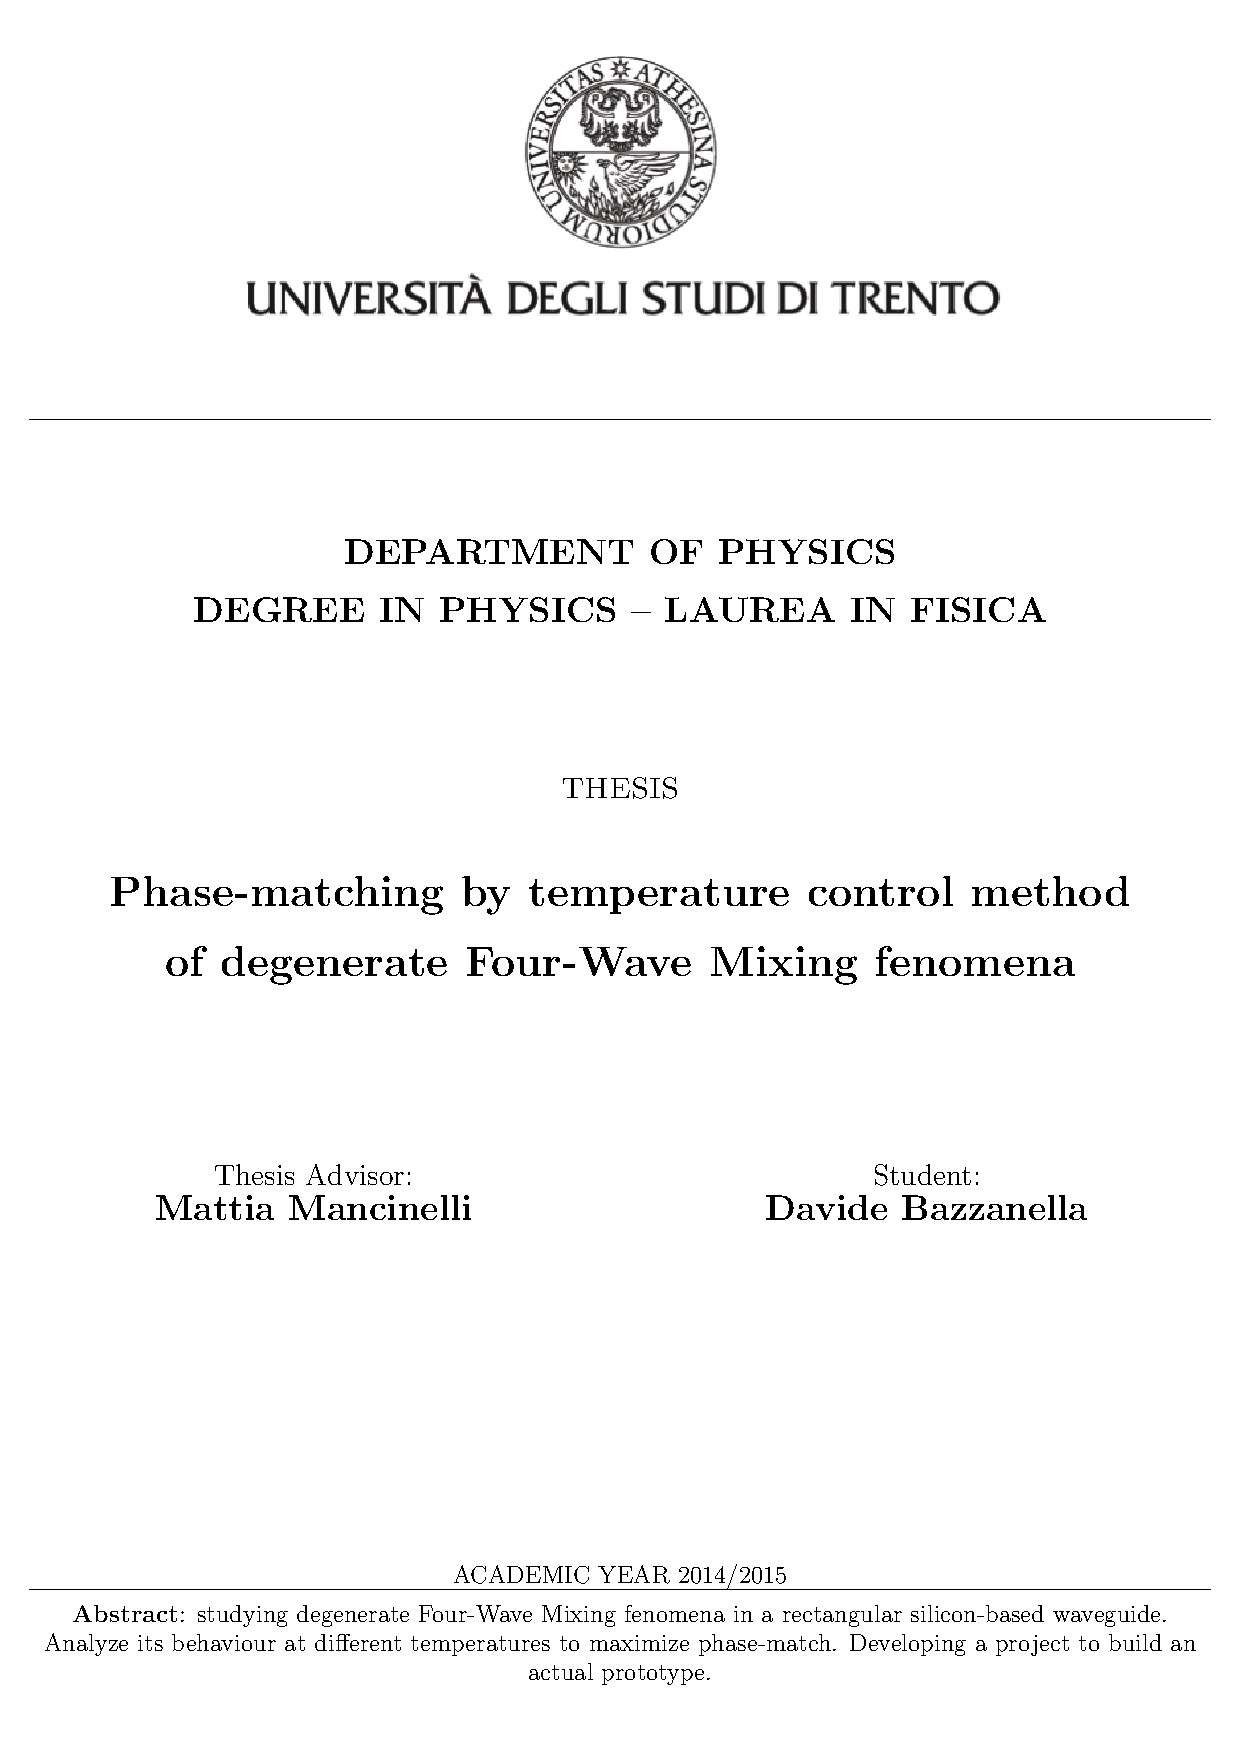
\includepdf[pages={1}]{intestazione.pdf} % \documentclass[11pt,a4paper]{article}
\usepackage[utf8]{inputenc}
\usepackage[english]{babel}
\usepackage{amsmath}
\usepackage{amsfonts}
\usepackage{amssymb}
\usepackage{graphicx}
\usepackage{parcolumns}
\usepackage[left=0.5cm,right=.5cm,top=.5cm,bottom=.5cm]{geometry}

\begin{document}

\begin{titlepage}
\begin{center}


\includegraphics[width=0.7\textwidth]{unitn_logo.png}~\\[1.2cm]

\hrule
$$$$
$$$$

\textsc{\LARGE \textbf{DEPARTMENT OF PHYSICS}}\\[0.5cm]
\textsc{\LARGE \textbf{DEGREE IN PHYSICS – LAUREA IN FISICA}}\\[2.5cm]
\textsc{\Large THESIS}\\[1.3cm]

{ \huge \bfseries Phase-matching by temperature control method}\\
[0.5cm]
{ \huge \bfseries of degenerate Four-Wave Mixing fenomena}\\
[3.0cm]

% ATTENZIONE! Ha bisogno del pacchetto parcolumns per funzionare
\begin{parcolumns}{2}
   \colchunk{\Large Thesis Advisor:\\ \LARGE \textbf{Mattia Mancinelli}}
   \colchunk[2]{\Large Student:\\ \LARGE \textbf{Davide Bazzanella}}
\end{parcolumns}
$$$$
$$$$
$$$$
$$$$
$$$$
$$$$
$$$$
$$$$

\large ACADEMIC YEAR 2014/2015
\hrule
\vfill
\textbf{Abstract}: studying degenerate Four-Wave Mixing fenomena in a rectangular silicon-based waveguide. Analyze its behaviour at different temperatures to maximize phase-match. Developing a project to build an actual prototype.

\vfill

{\large}

\end{center}
\end{titlepage}

\end{document}

\cleardoublepage 
\setcounter{page}{3}
\tableofcontents

\cleardoublepage
\pagenumbering{arabic}

\section{Introduction}
\subsection{Motivation}
In my academic career I first approached the study of optics during an elective course of my third year of undergraduate academic degree.
I became very interested in the subject, in particular because of the potential developement of photonics for communications and computing.
I discussed different topics with several professors and researchers.
One of the researchers, who would later become my advisor, suggested me a few interesting topics in guided-wave optics which could be studied in an undergraduate thesis.

I chose to study the temperature behaviour of silicon waveguides.
The reason of this choice is the constant presence of discrepancies between the design of silicon objects and their actual industrial production.
The aim of the study is to exploit behaviour of silicon to correct these possible production defects of the materials.

The study is focused on a silicon-based waveguide with a silicon ($\mathrm{Si}$) core of rectangular section and a silica ($\mathrm{SiO}_2$) cladding.
The purpose of the waveguide is to generate light through a partial degenerate Four-Wave Mixing phenomenon.

\subsection{Partially degenerate Four-Wave Mixing}
Four-Wave Mixing (FWM) is a nonlinear optical effect due to the susceptibility of silicon.
Silicon is an isotropic material and therefore second order susceptibility $\chi^{(2)}$ (almost) vanishes.
Third order susceptibility $\chi^{(3)}$, on the other hand, is non-zero and is responsible among the other effects for FWM, which is indeed a third order phenomenon.

In general FWM implies the mixing of four waves of different frequencies.
Partial degenerate FWM, instead, is a specific case where two waves have the same frequency and are considered as one (pump).
Therefore it is about the pump wave and a second weaker one (signal) which generate a third wave (idler) of frequency different from that of the former two.

\section{Electromagnetic waves in dielectric media}

%pg 156 saleh or chp 2 agrawal
To understand electromagnetic phenomena the starting point is the well known Maxwell's equations:
\begin{subequations}
\begin{align}
	\nabla \times \textbf{E} &= -\frac{\partial \textbf{B}}{\partial t}
		\label{eq_maxwell_a} \\
	\nabla \times \textbf{H} &= \textbf{J} + \frac{\partial \textbf{D}}{\partial t}
		\label{eq_maxwell_b} \\
	\nabla \cdot \textbf{D} &= \rho_{\mathrm{f}} 
		\label{eq_maxwell_c} \\
	\nabla \cdot \textbf{B} &= 0
		\label{eq_maxwell_d}
\end{align}
\end{subequations}
where \textbf{E} and \textbf{H} are electric and magnetic field vectors and \textbf{D} and \textbf{B} are corresponding electric and magnetic flux densities. \textbf{J} is the current density vector and $\rho_{\mathrm{f}}$ is the free charge density.
In dielectric media, such as silicon, we can also consider $\textbf{J} = 0$ and $\rho_\mathrm{f} = 0$.

\textbf{D} and \textbf{B} are related to the electromagnetic fields through the relations:
\begin{subequations}
\begin{align}
	\textbf{D} &= \varepsilon_0 \textbf{E} + \textbf{P} \\
	\textbf{H} &= \mu_0 \textbf{H} + \textbf{M}	
\end{align}
\end{subequations}
where $\varepsilon_0$ is the vacuum permittivity, $\mu_0$ is the vacuum permeability, and \textbf{P} and \textbf{M} are the induced electric and magnetic polarizations repectively.
For a nonmagnetic medium, as in our case, $\textbf{M} = 0$.

\subsubsection*{Solution in linear dielectric medium}
A linear dielectric medium is characterized by a linear relation between the polarization density and the electric field:
\begin{equation}
	\textbf{P} = \varepsilon_0 \chi \textbf{E}
	\label{eq_P_L}
\end{equation}
where $\chi$ is the susceptibility of the medium and $\varepsilon_r \equiv 1+\chi$ is the relative dielectric constant.

Taking the curl of Eq. (\ref{eq_maxwell_a}) and substituting it in Eq. (\ref{eq_maxwell_c}) leads to the Helmholtz equation:
\begin{equation}
\nabla^2 \textbf{E} - \frac{1}{c^2}\frac{\partial^2 \textbf{E}}{\partial t^2} = \mu_0\frac{\partial^2 \textbf{P}}{\partial t^2}
\label{eq_helm_P}
\end{equation}
where $c = 1/\sqrt{\mu_0 \varepsilon_0}$ is the speed of light in vacuum.

Defining the refractive index of the material $n \equiv \sqrt{\varepsilon_r}$ and using the definition of \textbf{P} as in Eq. (\ref{eq_P_L}), the previous Eq. (\ref{eq_helm_P}) becomes
\begin{equation}
	\nabla^2 \textbf{E} - \frac{n^2}{c^2}\frac{\partial^2 \textbf{E}}{\partial t^2} = 0
	\label{eq_helm_lin}
\end{equation}
Moreover, $n$ represents the ratio between the speed of light in vacuum and in the material ($n = c/v$) and it depends on the frequency of the EM wave.

The general solution of Eq. (\ref{eq_helm_P}) is a transverse electromagnetic (TEM) wave, whose electric and magnetic fields are perpendicular to the direction of propagation.
Without losing generality, we could assume $\hat{z}$ as the propagation direction and an electric field of the form:
\begin{equation}
	\textbf{E} = \frac{1}{2}\hat{x}\,E\,\mathrm{exp}[\mathrm{i}(kz-\omega t)] + c.c.
	\label{eq_wave}
\end{equation}
with $E$ amplitude of the electric field, $k = 2\pi/\lambda$ the wavevector and $\omega = 2\pi f$ the angular frequency.
$\lambda$ and $f$ are respectively the wavelength and the frequency of the electromagnetic wave.
The magnetic field has a similar equation.

\subsection{Silicon waveguides}
In linear optics the technology for trasmitting a light wave by confining it in a finite space is called guided-wave optics.
The instruments employed for achieving such purpose are called waveguides.

In a ray-optics picture, silicon waveguides are dielectric waveguides and make use of the interface between two media with different refractive index.
They exploit the phenomenon of total internal reflection: if a propagating wave reaches a boundary between two mediums, one with higher refractive index ($n_H$) and another with lower refractive index ($n_L$), with an angle of incidence greater than the \textit{critical angle}, then the wave is completely reflected in the first medium.
%accorciare la precedente frase%
Angles are defined relative to the normal vector of the interface and the critical angle can be obtained through the Snell's law:

$$	\theta_C = \arcsin \left( \frac{n_L}{n_H} \right)$$

Silicon waveguides are composed by core and cladding. %is called cladding only for fiber or also for slab/strip wg?
The former is the higher refractive index medium in which the wave is confined, the latter is the lower refractive index medium which surrounds the core, thus creating the interface. Theoretically, the cladding could also be vacuum.

\subsubsection*{Wave equation and modes}
Considering an ideal dielectric waveguide (no absorption) with the purpose of transmitting EM waves in the $\hat{z}$ direction, the total field distribution is a sum of continous TEM plane waves.
Defining the amplitude of the fields as $E(\textbf{r},t) = F(x,y)A(z,t)$ and $k=\beta$ and substituting them in Eq. (\ref{eq_wave}) leads to the following equation:
\begin{equation*}
	\textbf{E} = \frac{1}{2}\hat{x}\,F(x,y)A(z,t)\,\mathrm{exp}[\mathrm{i}(\beta z-\omega t)] + c.c.
\end{equation*}

The previous equation represents what is called a ``transverse electric" (TE) wave.
A second family of solutions could be acquired by defining the sum of TEM waves with the magnetic field always perpendicular to the propagation direction.
This is called a ``transverse magnetic" (TM) wave.

Is then possible to study the propagation of the wave along the waveguide using the Helmholtz equation (\ref{eq_helm_P}) or (\ref{eq_helm_lin}), obtaining the next equations:

\begin{subequations}
\begin{align}
	\frac{\partial^2F(x,y)}{\partial x^2} + \frac{\partial^2F(x,y)}{\partial y^2} + \left[ k_0^2n^2(x,y)-\beta^2\right]F(x,y) = 0
	\label{eq_wg_a} \\
	\frac{\partial^2\tilde{A}(z,\omega)}{\partial z^2} +2\mathrm{i}\beta\frac{\partial \tilde{A}(z,\omega)}{\partial z} -n^2k_0^2\tilde{A}(z,\omega) = 0
	\quad ! \neq ! \quad
	2\mathrm{i}\beta_0\frac{\partial \tilde{A}(z,\omega)}{\partial z} +(\tilde{\beta}^2 - \beta_0^2)\tilde{A}(z,\omega) = 0
	\label{eq_wg_b}
\end{align}
\end{subequations}
where $k_0$ is the wavevector in vacuum and $n=n(x,y)$ is a function of the position (mainly $x$ and $y$ for a straight waveguide).

The first equation, once solved, leads to the field distribution $F(x,y)$ in the plane perpendicular to the waveguide axis ($\hat{z}$).
Its solution is strictly linked to the geometry of the waveguide and to the dependence of the refractive index $n$ to the position in the plane.

The second equation (\ref{eq_wg_b}), on the other hand, defines the change in field distribution along the $\hat{z}$ axis, or the waveguide axis.
Imposing this equation to be zero means that we force the field distribution $F$ not to change.
%Indeed not all field distributions are transmitted through the waveguide without energy loss \textbf{(?)} and thus without changing $F$.
% Modes are fields that maintain the same transverse distribution and polarization at all locations along the waveguide axis.
Those field distributions which maintain the same transverse distribution and polarization at all locations along the waveguide axis are called modes.
These modes are the eigenfunctions of the system.
They can be categorized in two main groups, according to the polarization of the wave: transverse electric (TE) modes and transverse magnetic (TM) modes, which have respectively the electric and magnetic field transverse to the waveguide axis.

Solving for $\beta$, we obtain that only a discrete set of values $\beta_m$ verify the equation.
Replacing those values in Eq. (\ref{eq_wg_a}), leads to the field distribution F(x,y) to be defined.
Therefore both TE and TM modes can be again classified by their order, that is proportional to the number of maxima of the modulus of the electric and magnetic fields in the core section.
The first order has only one maximum at the center of the core, the second order has two maxima placed simmetrically from the center and so on.

Moreover it is noteworthy that the field distributions of even orders are even functions and those of odd orders are odd functions.

\begin{figure}[ht]
	\centering
	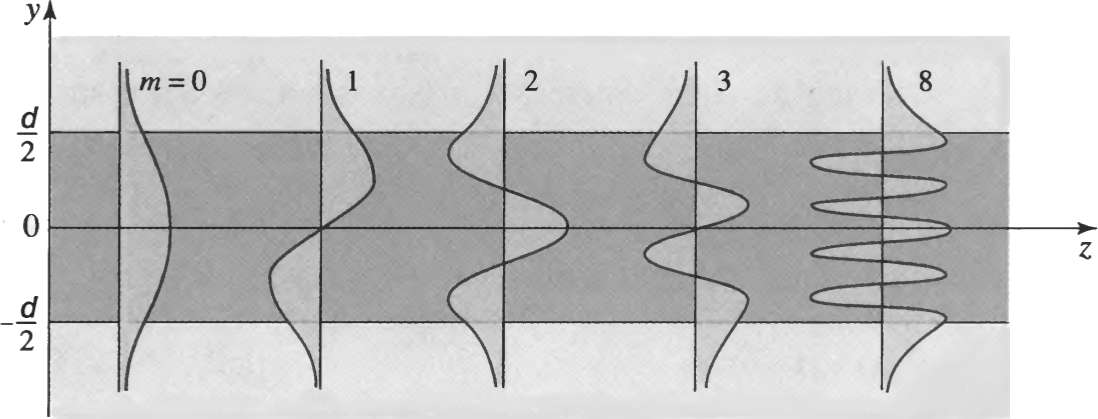
\includegraphics[width=.75\textwidth]{1D_fields.png}
	\label{fig_1dmodes}
	\caption{graphical rapresentation of field distribution of 1D modes}
\end{figure}

\subsubsection*{Propagation constant and effective index}

A very important parameter of each mode is its \textit{propagation constant} $\beta$, defined as the component of the wavevector $k$ in the waveguide axis:
\begin{equation}
\beta \equiv k|_z
\end{equation}

Higher-order modes travel with smaller propagation constants.
Considering the simplest case: a 1D waveguide, which has a planar core of thickness $d$ and cladding over and under it expanding to infinite.
For this waveguide, also called a \textit{slab}, $\beta$ has a simple relation with the bounce angles $\theta_m$, which are quantized between $0$ and $\bar{\theta}_C = \pi - \theta_C$:
$$\beta_m = n_H k_0 \cos \theta_m$$

From the propagation constant, we can also define the refractive index relative to the propagation mode, called \textit{effective index}:
\begin{equation}
\beta = k_0 n_{eff} \quad \Rightarrow \quad n_{eff} \equiv \frac{\beta}{k_0}
\end{equation}

Its value is between the higher index of the core and lower one of the cladding.
Again, for the 1D slab waveguide case, the effective index can be rewritten as in the following formula:
$$ n_{eff} \equiv n_H \cos \theta_m$$

\begin{figure}[!hb]
	\centering
	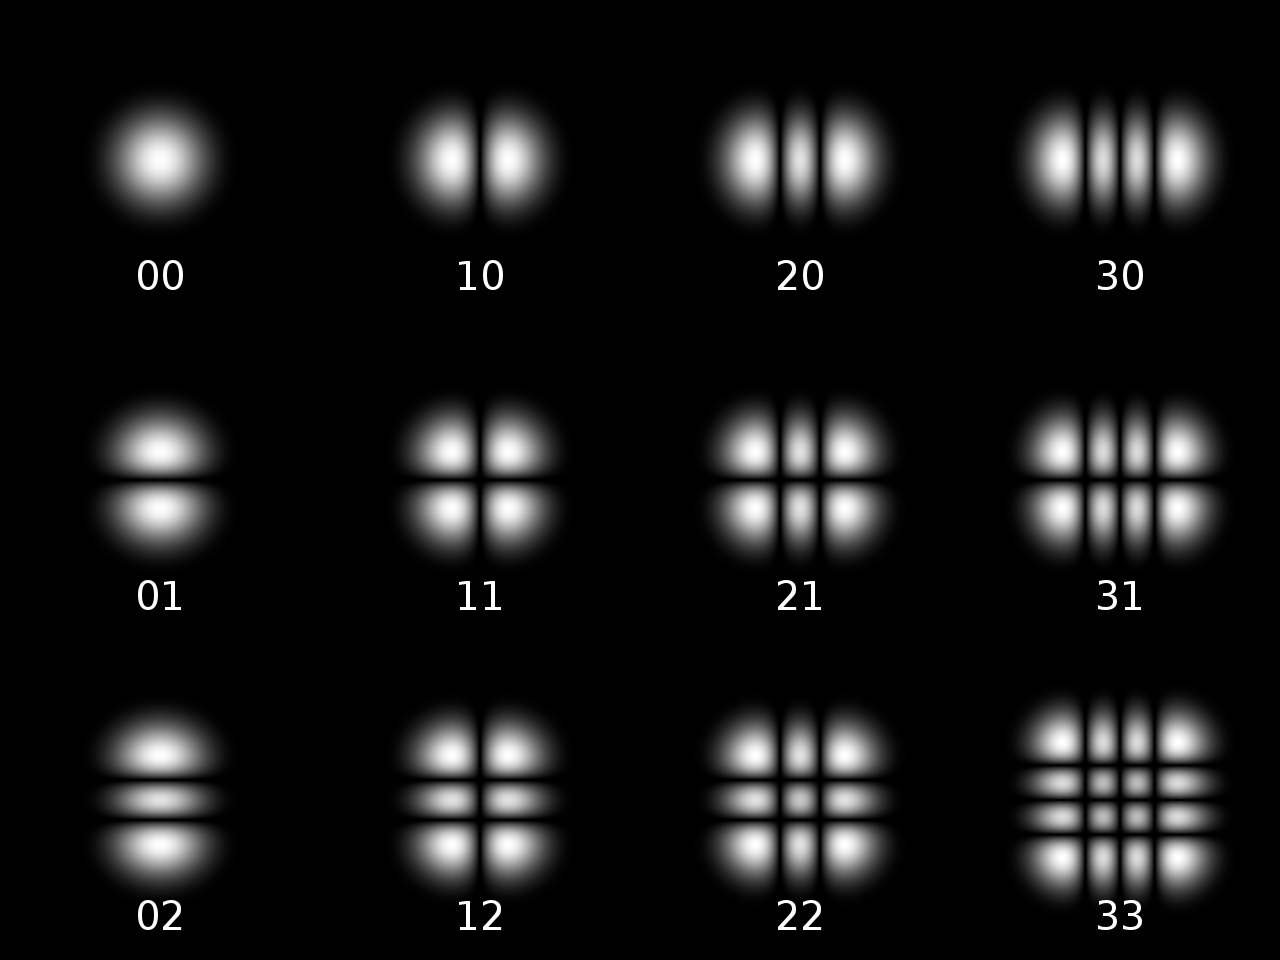
\includegraphics[width=.45\textwidth]{2Dmodes.png}
	\caption{Graphical rapresentation of field distribution of 2D modes}
	\label{fig_2dmodes}
\end{figure}

\subsection{Rectangular dielectric waveguides}
In general, in a rectangular dielectric waveguide the classification of modes need two indexes because we have two degrees of freedom.
In Figure (\ref{fig_2dmodes}) is graphically represented the distribution of the fields in modulus.

For our purpose, due to the thin geometry of the core, the waveguide does not support modes with the higher order in the height axis than the fundamental one.
The first row is of our interest.
Only one significant index is then left to describe the order of modes.

\section{Non-linear optics}

\begin{figure}[!ht]
	\centering
	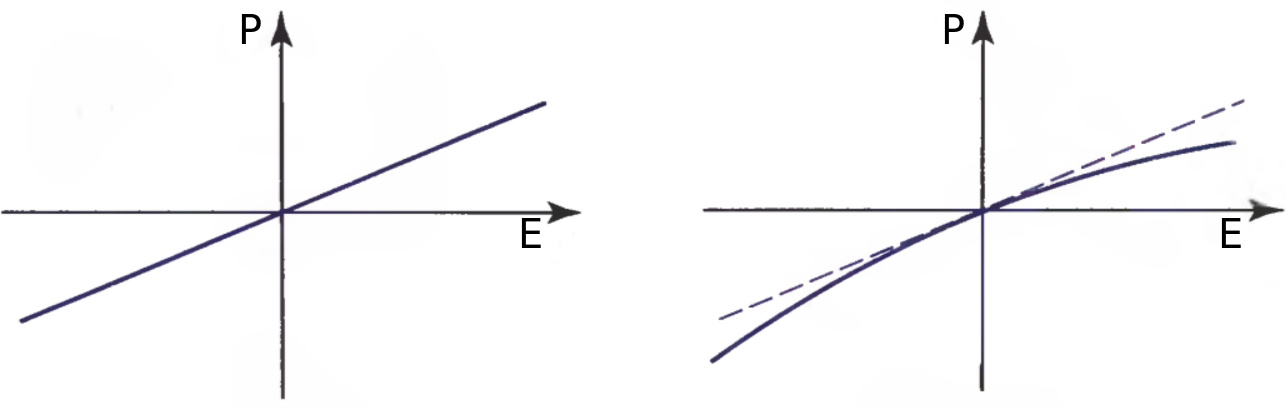
\includegraphics[width=.75\textwidth]{nonlinearity.png}
	\caption{Example of nonlinear relation between \textbf{P} and \textbf{E}}
	\label{fig_nonlinearity}
\end{figure}

A nonlinear dielectric medium is characterized by a nonlinear relation between \textbf{P} and \textbf{E}, such as
\begin{equation}
	\textbf{P} = \varepsilon_0 \left( \chi^{(1)} \cdot \textbf{E} + \chi^{(2)} : \textbf{E}^2 + \chi^{(3)} \vdots \textbf{E}^3 + \cdots \right) = \mathrm{\textbf{P}_L} + \mathrm{\textbf{P}_{NL}}
	\label{eq_P_general}
\end{equation}
which originates from the behaviour of bound electrons.

In everyday conditions linear effects are much larger than nonlinear ones.
The relation between \textbf{P} and \textbf{E} becomes nonlinear when $\mathrm{E}$ has a value comparable to interatomic electric fields, which are typically $\sim 10^5-10^8$ \si{\V\per\m}.

For an isotropic medium the second order term is zero (in the dipole approximation) and this is our scenario.
Thus the dominant nonlinearity is the third order and the material is called a Kerr medium.

\subsection{Third order effect: Four-Wave Mixing}
Many processes are result of third order nonlinearities: Third-Harmonic Generation (THG), Kerr Effect, Cross-phase modulation (XPM), Self-phase modulation (SPM) and Four-Wave Mixing (FWM).

The parametric process of Four-Wave Mixing originates from the third order nonlinear response of a material to an electromagnetic field and involves interaction among four optical waves.

Considering significant only the third-order term, the nonlinear component of the induced electric polarization vector is
\begin{equation}
	\textbf{P}_{NL} = \varepsilon_0 \chi^{(3)} \vdots \textbf{E}^3
	\label{eq_P_NL}
\end{equation}

Considering a silicon waveguide with a rectangular core section, to study the propagation of four waves, the total electric field can be expressed as
\begin{equation}
	\textbf{E} = \frac{1}{2}\hat{x} \sum_{j=1}^4 E_j \mathrm{exp}[i(\beta_j z - \omega_j t)] + c.c.
	\label{eq_E}
\end{equation}

Substituting Eq. (\ref{eq_P_NL}) in Eq. (\ref{eq_E}) we obtain $8^3=512$ terms.
We can then write the non linear terms $\mathrm{\textbf{P}_{NL}}$ of the induced electric polarization as
\begin{equation}
	\mathrm{\textbf{P}_{NL}} = \frac{1}{2}\hat{x} \sum_{j=1}^4 P_j \mathrm{exp}[i(\beta_j z - \omega_j t)] + c.c.
	\label{eq_P}
\end{equation}

where for example $P_4$ would be
\[
\begin{array}{rl}
	P_4 &= \frac{3\varepsilon_0}{4} \chi^3_{xxxx}\left[ |\mathrm{E}_4|^2\mathrm{E}_4 2(|\mathrm{E}_1|^2+|\mathrm{E}_2|^2+|\mathrm{E}_3|^2)\mathrm{E}_4 \right. \\
	&+ \left. 2\mathrm{E}_1\mathrm{E}_2\mathrm{E}_3\mathrm{e}^{i\phi_+}+2\mathrm{E}_1\mathrm{E}_2\mathrm{E}_3^*\mathrm{e}^{i\phi_-} + ...\right]\\

\end{array}
\]
\hspace{18pt}with $\phi_+$ and $\phi_-$ defined as
\[
\begin{array}{lr}
\phi_+ &= (\beta_1+\beta_2+\beta_3-\beta_4+)z - (\omega_1+\omega_2+\omega_3-\omega_4)t \\
\phi_- &= (\beta_1+\beta_2-\beta_3-\beta_4+)z - (\omega_1+\omega_2-\omega_3-\omega_4)t \\
\end{array}
\]

Significant FWM occurs only if the phase match nearly vanishes.
This requires the matching of frequencies as well as of the wave vectors.
Thus the phase-matching condition requires a specific choice of input wavelengths and media parameters before FWM can occur with high efficiency.

From the definition of $\phi_-$ and $\phi_+$ we can gather that there are two types of FWM.
The term containing $\phi_-$ corresponds to the case in which two photons at frequencies $\omega_1$ and $\omega_2$ are annihilated, while two photons at frequencies $\omega_3$ and $\omega_4$ are created simultaneously.
On the other hand, the term containing $\phi_+$ corresponds to the case in which three photons at frequencies $\omega_1$, $\omega_2$ and $\omega_3$ are annihilated, while one photon at frequency $\omega_4$ is created.

Our study focuses on a special condition of the second case, where $\omega_1 = \omega_2 = \omega_P$. The setup therefore consists of a strong pump of frequency  $\omega_P$ and a signal of frequency  $\omega_3 = \omega_S$, resulting in the creation of the idler wave of frequency $\omega_4 = \omega_I$, as in Figure (\ref{fig_setup}).
The condition of frequency and phase matching are therefore:
\begin{equation}
\left\{
 	\begin{aligned}
		\omega_I &= 2\omega_P - \omega_S \\
		\Delta k &= 2\beta_P - \beta_S - \beta_I = 0
	\end{aligned}
\right.
\label{eq_f&pmc}
\end{equation} %frequency & phase matching conditions

\begin{figure}[ht]
	\centering
	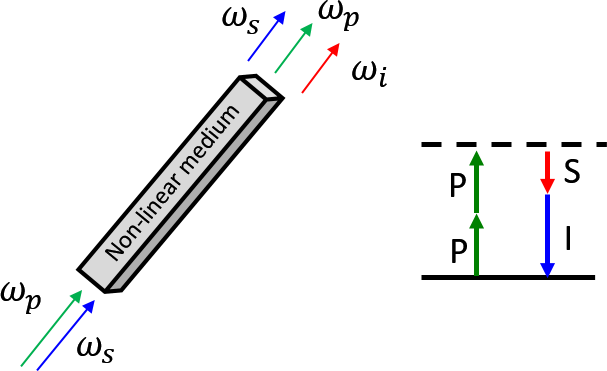
\includegraphics[width=.55\textwidth]{setup.png}
	\caption{Symbolical rapresentation of the setup}
	\label{fig_setup}
\end{figure}


\subsubsection{Coupled amplitude equations}

Replacing Eq. (\ref{eq_P}) in the Helmholtz equation (\ref{eq_helm_P}) leads to eight coupled equations: four of them are equivalent of Eq. (\ref{eq_wg_a}) and describe the field distribution of the mode of each wave.
The remaining four are the equivalent of Eq. (\ref{eq_wg_b}) and describe how the fields change while travelling through the waveguide.
Considering $E_j(\textbf{r}) = F_j(x,y)A_j(z)$ where $F_j$ is the spatial distribution of the mode, they can be written as:

\begin{subequations}
\begin{align}
	\frac{dA_1}{dz} &= \frac{\mathrm{i}n_L\omega_1}{c}\left[ \left( f_{11} |A_1|^2 + 2 \sum_{k\neq1} f_{1k}|A_k|^2\right)A_1 + 2f_{1234}A_2^*A_3A_4\mathrm{e}^{+\mathrm{i}\Delta k_z} \right]
		\label{eq_coupled_amplitude_a}\\
	\frac{dA_2}{dz} &= \frac{\mathrm{i}n_L\omega_2}{c}\left[ \left( f_{22} |A_2|^2 + 2 \sum_{k\neq2} f_{2k}|A_k|^2\right)A_2 + 2f_{2134}A_1^*A_3A_4\mathrm{e}^{+\mathrm{i}\Delta k_z} \right]
		\label{eq_coupled_amplitude_b}\\
	\frac{dA_3}{dz} &= \frac{\mathrm{i}n_L\omega_3}{c}\left[ \left( f_{33} |A_3|^2 + 2 \sum_{k\neq3} f_{3k}|A_k|^2\right)A_3 + 2f_{3412}A_1A_2A_4^*\mathrm{e}^{-\mathrm{i}\Delta k_z} \right]
		\label{eq_coupled_amplitude_c}\\
	\frac{dA_4}{dz} &= \frac{\mathrm{i}n_L\omega_4}{c}\left[ \left( f_{44} |A_4|^2 + 2 \sum_{k\neq4} f_{4k}|A_k|^2\right)A_4 + 2f_{4321}A_1A_2A_3^*\mathrm{e}^{-\mathrm{i}\Delta k_z} \right]
		\label{eq_coupled_amplitude_d}
\end{align}
\label{eq_coupled}
\end{subequations}

where
\begin{equation}
	f_{ij} = \frac{\langle |F_i|^2 |F_j|^2 \rangle}{\sqrt{\langle |F_i|^2 \rangle\langle |F_j|^2 \rangle}}
\end{equation}
\hspace{18pt}and
\begin{equation}
	f_{ijkl} = \frac{\langle F_i^* F_j^* F_k F_l \rangle}{\sqrt{\langle |F_i|^2 \rangle\langle |F_j|^2 \rangle\langle |F_k|^2 \rangle\langle |F_l|^2 \rangle}}
\end{equation}
\hspace{18pt}are the overlap integrals of the different modes, where the brackets mean an integration on a plane $\langle g(x,y)\rangle = \int\int_{-\inf}^{\inf}g(x,y)\mathrm{dxdy}$.
The physical interpretation of such quantities is how much different modes are overlapped with each others.

\subsubsection{Approximate solution}
The previous equations are quite general (they include SPM, XPM in addition to FWM) and require a numerical approach to be solved exactly.
For this reason, we propose an approximate solution to understand the physical implications.
The first approximation is called ``undepleted pump" and consists in assuming the pump waves to be much more intense than the other waves.
As a further simplification, we assume that all overlap integrals are nearly the same
\begin{equation}
	f_{ijkl} \approx f_{ij} \approx \frac{1}{A_{eff}}	\qquad \qquad i,j,k,l = 1,2,3,4
	\label{eq_overlap_approx}
\end{equation}
From this definition follows naturally the nonlinear parameter definition
\begin{equation}
	\gamma_j = \frac{n_2\omega_j}{cA_{eff}} \approx \gamma
	\label{eq_gamma_approx}
\end{equation}
where $\gamma$ is the average value (because frequencies have relatively small differencies).

Using the last two equations and the undepleted pump approximation, (\ref{eq_coupled_amplitude_a}) and (\ref{eq_coupled_amplitude_b}) are easily solved to obtain the pump fields
\begin{subequations}
\begin{align}
	A_1(z) &= A_1(0)\mathrm{exp}[\mathrm{i}\gamma(P_1 + 2P_2)z] \\
	A_2(z) &= A_2(0)\mathrm{exp}[\mathrm{i}\gamma(P_2 + 2P_1)z]
\end{align}
	\label{eq_pump_sol}
\end{subequations}
where $P_j = |A_j(z=0)|^2$.

Using the same approximations on (\ref{eq_coupled_amplitude_c}) and (\ref{eq_coupled_amplitude_d}) and replacing Eqs (\ref{eq_pump_sol}a) and (\ref{eq_pump_sol}b) where needed we obtain two linear coupled equations for signal and idler:
\begin{subequations}
\begin{align}
	\frac{dA_3}{dz} &= 2\mathrm{i}\gamma [(P_1 + P_2)A_3 + A_1(0)A_2(0)\mathrm{e}^{-\mathrm{i}\phi}A_4^*]
	\label{eq_sig}\\
	\frac{dA_4}{dz} &= 2\mathrm{i}\gamma [(P_1 + P_2)A_4 + A_1(0)A_2(0)\mathrm{e}^{-\mathrm{i}\phi}A_3^*]
	\label{eq_idl}
\end{align}
\end{subequations}
where $\phi = [\Delta k - 3\gamma(P_1 + P_2)]z$.

These equations can be solved introducing $B_j = A_j \,\mathrm{exp}[-2\mathrm{i}\gamma(P_1+P_2)z]$ for $j=3,4$ giving their general solution as
\begin{equation*}
	B_j(z) = (a_j\mathrm{e}^{gz}+b_j\mathrm{e}^{-gz})\mathrm{exp}(-i\kappa z/2)
\end{equation*}
with $\kappa = \Delta k + \gamma(P_1 + P_2)$ \textit{effective phase mismatch} and $g = \sqrt{4\gamma^2P_1P_2 - \kappa^2/4}$ the \textit{parametric gain}.

The solutions of Eqs (\ref{eq_sig}) and (\ref{eq_idl}) are therefore
\begin{subequations}
\begin{align}
	A_3(z) &= \left(a_3\mathrm{e}^{gz}+b_3\mathrm{e}^{-gz}\right)\mathrm{exp}\left[-\frac{\mathrm{i}}{2}(\Delta k -3\gamma(P_1 + P_2))z\right]
		\label{eq_sig_sol} \\
	A_4(z) &= \left(a_4\mathrm{e}^{gz}+b_4\mathrm{e}^{-gz}\right)\mathrm{exp}\left[-\frac{\mathrm{i}}{2}(\Delta k -3\gamma(P_1 + P_2))z\right]	
		\label{eq_idl_sol}
\end{align}
\end{subequations}

The solution that we have developed so far is valid only when the pump waves remain largely undepleted.
For a solution that includes pump depletion it is necessary to solve exactly the complete set of four equations, Eqs (\ref{eq_coupled_amplitude_a} - \ref{eq_coupled_amplitude_d}).

We can also define a length scale, known as the coherence length, using $L_{coh} = 2\pi/|\Delta\kappa|$, where $\Delta\kappa$ is the maximum value of the effective phase mismatch that can be tolerated.
Moreover significant FWM occurs if $L_{sam}<L_{coh}$ where $L_{sam}$ is the sample length.
This definition allow us to make a further assumption, that is $\kappa = \Delta k + \gamma(P_1 + P_2) \approx \Delta k$.
Considering a peak power $P_1+P_2 = \SI{1}{\W}$ of the pump and a sample length $L_{sam} = \SI{1}{\cm}$ we obtain
\begin{equation*}
\left\{
 	\begin{aligned}
		\gamma(P_1 + P_2) &= \frac{n_2\omega}{cA_{eff}}P_0 = \frac{\SI{4.5e-18}{\m^2\per\W}}{c\SI{e-12}{\m^2}}\frac{2\pi c}{\SI{1.55e-6}{\m}}\SI{1}{\W} \approx \SI{20}{\per\m} \approx \SI{e1}{\per\m}\\
		|\Delta k |&= \frac{2\pi}{L_{sam}} = \frac{2\pi}{\SI{1}{\cm}} \approx \SI{600}{\per\m} \approx \num{e2} - \SI{e3}{\per\m}
	\end{aligned}
\right.
\label{eq_f&pmc}
\end{equation*}

since $|\Delta k| \gg \gamma(P_1 + P_2)$ almost always we can consider it trascurable.

Therefore, in order to be efficient, the parametric process needs to verify the conservation of both energy and momentum, as given in Eq. (\ref{eq_f&pmc}).

\section{Computational model}

Our aim is to study how the generation of a new wave at different frequency through FWM is influenced by the different modes of the waveguide.
Waveguide modes indeed react differently to the change of frequency and temperature of the system, which are the free variables of the problem.

To understand the behaviour of the waveguide, it is first necessary to know how waves of different frequencies are transmitted through the waveguide.
We chose to simulate the modes with temperature and frequency as a parameters.

Our aim was to develop a model to work with an infrared laser pump with $\lambda_{p} = \SI{1.55}{\um}$.
The reasons are that silicon is transparent at these wavelength and also that lasers that emit at the specific wavelength are largely available.

We narrowed our simulations to a frequency gap centered in $\omega_p = 2\pi \nu_p = 2\pi c / \lambda_{p}$.
The gap chosen was precisely $[\SI{1.45}{\um} ,\, \SI{1.65}{\um}]$ or the equivalent $[\SI{182}{\THz} ,\, \SI{207}{\THz}]$, because we have tunable lasers which work in this spectral range.
The temperature gap, on the other hand, was chosen to be $[\SI{0}{\K} - \SI{400}{\K}]$ over ambient temperature $T_{amb} = \SI{293.15}{\K} = \SI{20}{\celsius}$, that is $[\SI{293.15}{\K} - \SI{693.15}{\K}]$. It is reasonable to heat the silicon up to \SI{400}{\celsius}.

\subsection{Simulation}
To obtain definite solutions, we had to assign the materials and a geometry to the problem first.

\begin{figure}[ht]
	\centering
	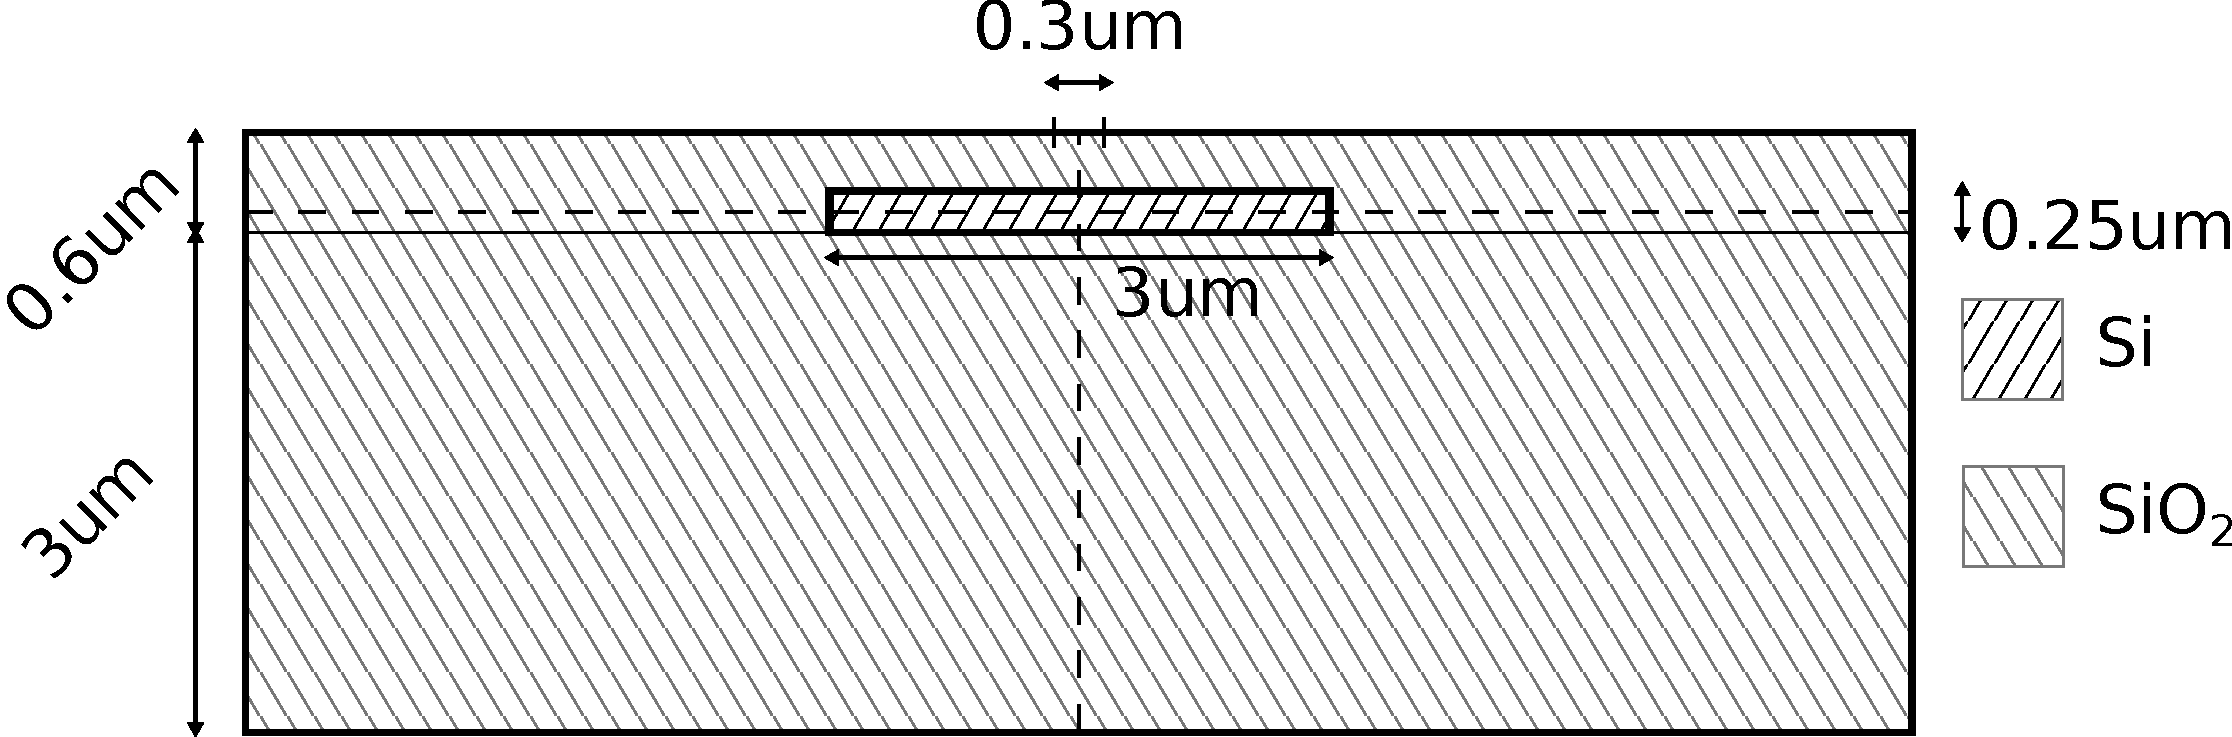
\includegraphics[width=1\textwidth]{geometry.pdf}
	\label{fig_wg_Section}
	\caption{Section of the rectangular waveguide}
\end{figure}

We modelled a dielectric waveguide with a silicon (Si) core \SI{3}{\um} wide and \SI{.25}{\um} high.
The cladding was set to be silica (SiO2) and coated the top of the core with a thickness of \SI{.35}{\um}.
For both materials was defined a refractive index dependent on the wavelength $n=n(\lambda)$, as given by the empirical relationship called \textit{Sellmeier equation}:
\begin{equation}
	n^2(\lambda) = 1+ \sum_i \chi_{0i}\frac{\lambda^2}{\lambda^2-\lambda^2_i}
	\label{eq_sellmeier}
\end{equation}
where the weights are defined experimentally and vary depending on the material.

We positioned a thermal reservoir, a ``\textit{heater}", \SI{0.3}{\um} wide at the top of the cladding, exactly over the center of the waveguide core and set to mantain a specific temperature $T_H$ in the gap $[\SI{293.15}{\K} - \SI{693.15}{\K}]$, given by the configuration chosen.
To solve the heat equation we defined the density $\rho$ in [\si{\kg\m^3}], the thermal conductivity $\kappa_{TH}$ in [\si{\W\per\m\per\K}] and the heat capacity $C_P$ in [\si{\J\per\kg\per\K}] of the different materials.

\begin{table}[ht]
\centering
  \begin{tabular}{lcccc}  
    \toprule
		& \multicolumn{3}{c}{Properties} \\
    \cmidrule(r){2-5}
    	\multirow{2}{*}{Materials}    & $\rho$ & $\kappa_{TH}$ & $C_P$ & TOC\\
  		& [\si{\kg\m^3}] & [\si{\W\per(\m\K)}] & [\si{\J\per(\kg\K)}] & [\si{\per\K}] \\
    \midrule
    Silicon (Si)			& 2329	& 130	& 700	& \num{1.87e-4}\\
    Silica (SiO$_2$)		& 2203	& 1.38	& 703	& 0\\
    \bottomrule
  \end{tabular}
  \label{tab_materials}
  \caption{Thermal properties of silicon and silica glass}
\end{table}

Moreover, in order to be influenced by the different temperatures, we had to add to the definition of refractive index of the silicon a term dependent on the temperature.
For our purpose this dependence can easily be considered linear:
\begin{equation}
n = n(\lambda)+\mathrm{TOC}\cdot (T-T_{amb})
\end{equation}
where $\mathrm{TOC}|_{\mathrm{Si}} = \SI{1.87e-4}{\per\K}$\cite{n_db} is called Termo-Optic Coefficient. The coefficient of silica glass is negligible and therefore was considered zero $\mathrm{TOC}|_{\mathrm{SiO}_2} \approx 0$.

\subsubsection{Numerical solution}
Since the degrees of freedom of the problem were too many, we resorted to automated algorithms which gave us a numerical, and therefore approximate, solution.

\paragraph{Heat transfer: stationary solution}
The first step was solving the equation for the heat transfer to obtain a stationary solution for each temperature in the gap.
That means to know the local temperature for each position in the core and in the cladding, for each initial setup.

It was necessary to set the boundary conditions: the two sides (left, right) and the bottom were considered as thermal reservoirs with a temperature $T = T_{amb} = \SI{293.15}{\K}$.
The top was, instead, split into three sections: the heater, as we explained previously, and the remaining two parts.
These were set to have a convective heat flux with air at ambient temperature.
Silica heat transfer coefficient was set to $\mathrm{HTC}_{\mathrm{SiO}_2} = \SI{5}{\W\per(\m^2\K)}$.

It is important to note that the value of the heat transfer coefficient can vary a lot depending on the air motion.
We considered the typical laboratory condition.

\paragraph{EM mode analysis}

The second step was to find the different modes of the waveguide for each set of parameters, such as temperature and wavelength.

We employed an automated FEM algorithm to solve, in the frequency domain, the Helmholtz equation on a fine grid in the waveguide section.
Each point of evaluation took into account the effective index of the material, slightly changed by the local temperature obtained by the stationary solution.

As in the stationary solution of the heat transfer, we needed the boundary conditions.
We set all four sides (top, bottom, left, right) to ``\texttt{scattering boundary condition}", which is a condition where the boundary is completely transparent to scattered waves.
That means that the core and cladding is isolated from the outside.

This algorithm was set to find the eight modes whose effective index $n_{eff}$ was closest to $n_{eff}=4$ in absolute value.
\subsubsection{Data output}
We obtained the field distribution and a series of parameters as our data output for each parametric configuration.
In particular the parameters were the effective index $n_{eff}$, the effective area $A_{eff}$ and the nonlinear parameter $\gamma$, for each mode and for each wavelength and temperature.

\subsection{Data classification}
The next step was to classify these data, depending on the type (TE or TM) and order (1,2,3...) of the modes.
We achieved this by analyzing a sample taken at $y=0$ of the field distributions.
The ratio between the maxima values of the x-component and y-component of the electric field allowed to distinguish the mode type: TE or TM.
Those fields which had the maximum component in the y direction were categorized as TE modes while those which had the maximum component in the x direction as TM modes.
The number of maxima of the modulus of the field showed us the order of the mode.

We obtained then a well organized data matrix filled with the value of effective index $n_{eff}$, effective area $A_{eff}$ and nonlinear parameter $\gamma$ for each combination of parameters.

\subsection{Data processing}
We focused on the information given by the effective index.

\subsubsection{Polynomial fit}
Starting from raw data consisting of the effective index for each parametric configuration, we fitted them with a polinomial function of frequency $\omega = 2\pi \nu$ or $\lambda$ and temperature $T$, obtaining:
$$n_{eff} = f_{mt,\,mo} \left( \omega, T_H \right) = f'_{mt,\,mo} \left( \lambda, T_H \right)$$
where $mt$ and $mo$ means respectively \textit{mode type} (TE or TM) and \textit{mode order} (1, 2, 3, ...)

Specifically, we used a polynomial expression of fifth order in wavelength and second order in temperature ``\texttt{poly52}".

\subsubsection{Order combination}

Due to the intrinsic symmetry of the problem (and thus of the integrals) not all combinations of orders can produce FWM.
Only those in which the sum of the orders is an even number are interesting, because only in those combinations the overlap integrals in Eq. (\ref{eq_coupled}) are not zero.
To narrow the possible sets, we chose only full TE or full TM  combinations.

We eventually obtained a list of combinations and for each one we evaluated the phase mismatch.

\subsubsection{Conservation of energy and momentum}
As it is, the phase mismatch is a function of the wavelenghts of pump, signal and idler.
By imposing the conservation of energy,
\begin{equation}
2\omega_P = \omega_S + \omega_I
\qquad \Longrightarrow \qquad
\omega_I = 2\omega_P - \omega_S \\
\end{equation}
$$or \qquad \qquad \lambda_I = \left( \frac{2}{\lambda_P} - \frac{1}{\lambda_S}\right)^{-1} $$
we obtained the only frequency permitted for $\omega_I$.

We replaced its value in the conservation of momentum formula, giving us the phase mismatch as a function of signal wavelength and temperature of the heater only, for each set of orders.

%\begin{equation}
\begin{align*}
	\Delta k &= 2\beta_P(\omega_P)-\beta_S(\omega_S)-\beta_I(2\omega_P-\omega_S)\\
			 &= 2\pi\left[ 2\frac{n_{eff}^P(\lambda_P)}{\lambda_P}
			 - \frac{n_{eff}^S(\lambda_S)}{\lambda_S}
			 - \frac{n_{eff}^I(\lambda_I)}{\lambda_I}\right]
\end{align*}
%\end{equation}

Then, starting from the fits of the effective index at different wavelengths and temperatures, we evaluated the phase mismatch of all sets.
The evaluation was made on a grid of temperature and signal wavelength arbitrarily dense.

\subsubsection{Selection of sets}
Once evaluated all the points on the grid for all the sets available, we selected only the interesting combinations.
The critical parameter on which the choice was based on is the coherence length: only those sets which had a maximum value of coherence length greater than a supposed sample length $L_{sam} = $\SI{1}{\cm} was chosen.
\begin{equation}
	L_{coh} = \frac{2\pi}{|\Delta k|} \geq L_{sam}
	\label{eq_lcoh_crit}
\end{equation}
Again, we obtained a list containing only the combinations interesting for our purpose.

It is important to note that, in general, each combination could have more than one maximum of coherence length $L_{coh}$ in wavelength for each temperature value.

\begin{figure}[!h]
	\centering
	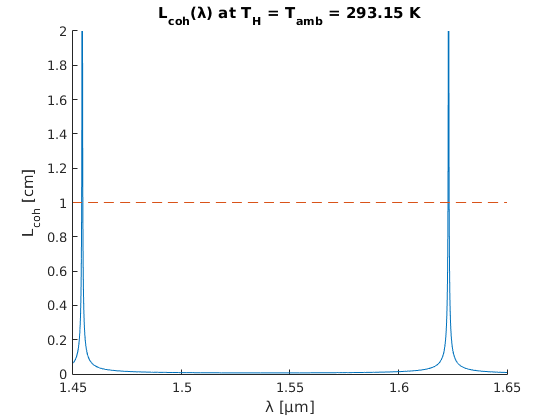
\includegraphics[width=.75\textwidth]{delta_example.png}
	\caption{Example of $L_{coh}$ at $T_H$ fixed.}
	\label{fig_peaks}
\end{figure}

\subsection{Data analysis}
We studied the value of $L_{coh}$ of the selected configurations with a rough analysis of 3D plots of $L_{coh}(\lambda,T_{H})$.
We observed the presence of different (mainly one or two) peaks in wavelength which were almost conserved in the temperature shift.

Given the definition of function $L_{coh}$, its value should technically diverge in the proximity of phase-match condition.
However, we evaluated the function on a discrete grid.
Thus we had, as a matter of fact, a very peaked function of wavelength most of the time.
An example is given in Figure (\ref{fig_peaks}).

We could therefore find the local maxima of such function and assume they are the centers of the peaks.
If their position changes significantly while shifting the temperature, it means we are able to control the phase-match condition.

Another important parameter is the width of the peak: to be consistent with the seletion criteria used in (\ref{eq_lcoh_crit}), we defined the bandwidth as the peak width at $L_{coh} = 1$.

We obtained graphs representing the position and the bandwidth of peaks vs temperature of each solution, as shown in Figures (\ref{fig_example_position}) and (\ref{fig_example_bandwidth}).

\begin{SCfigure}%[!h]
	\centering
	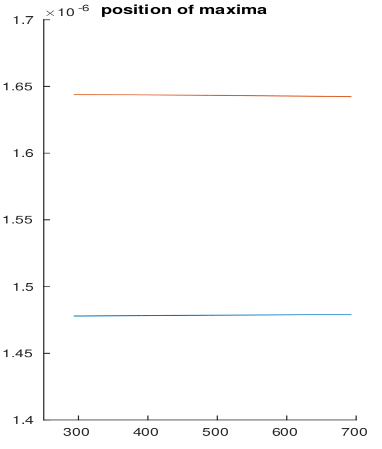
\includegraphics[width=.64\textwidth]{ex_pos.png}
	\caption{Example of peak position vs $T_H$.}
	\label{fig_example_position}
\end{SCfigure}
\begin{SCfigure}%[!h]
	\centering
%	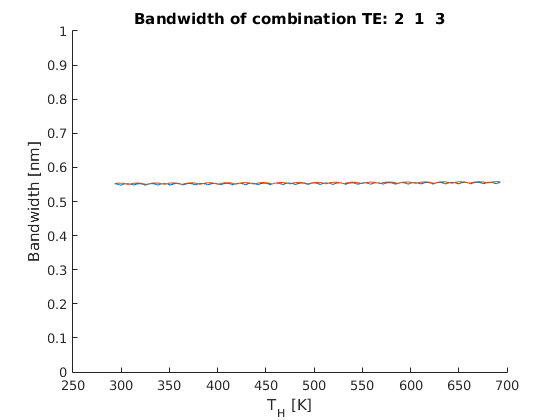
\includegraphics[scale=1]{ex_bw.png}
	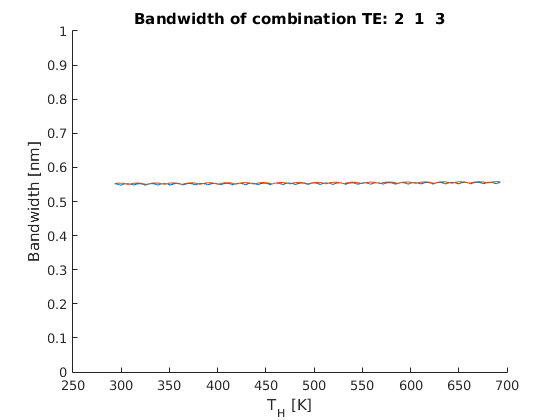
\includegraphics[width=.64\textwidth]{ex_bw.png}
	\caption{Example of bandwidth vs $T_H$.}
	\label{fig_example_bandwidth}
\end{SCfigure}

%\begin{figure}[!h]
%	\centering
%	\begin{subfigure}[b]{0.49\textwidth}
%		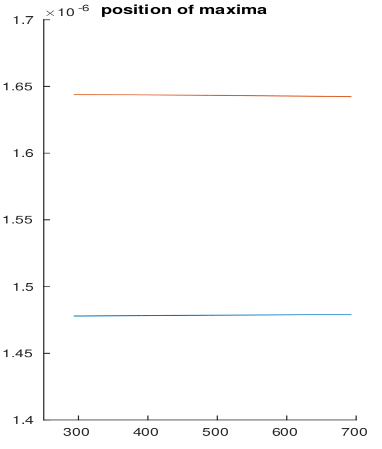
\includegraphics[width=1\textwidth]{ex_pos.png}
%		\caption{Example of peaks vs $T_H$.}
%		\label{fig_example_position}
%	\end{subfigure}%\hspace{.02\textwidth}
%	\begin{subfigure}[b]{0.49\textwidth}
%		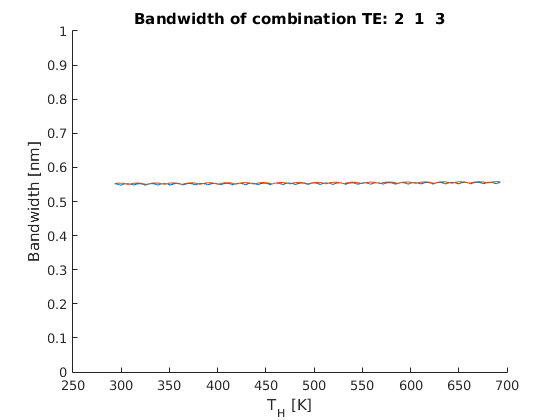
\includegraphics[width=1\textwidth]{ex_bw.png}
%		\caption{Example of bandwidth vs $T_H$.}
%		\label{fig_example_bandwidth}
%	\end{subfigure}
%	\caption{Examples of peaks position and bandwidth dependence on temperature $T_H$}
%	\label{fig_examples}
%\end{figure}

\section{Results}
\subsubsection{data aggregation}
Examining the graphs obtained from the data analysis of the symmetric configuration, we noticed that for each solution selected there were one or two straight lines.
Therefore we summarized them by collecting the slopes and the value of the functions at ambient temperature.
To make the graphs easier to read, we excluded set of data the pointsof no interest: those which peak had the same frequency $\omega_P = \SI{1.55}{\um}$ of the pump.

The first Figure (\ref{fig_sym_pp@t2}) tell us where we found phase-matching condition.
We can see that every set has its symmetric one.
For example, combination \texttt{517} is the symmetric of \texttt{571}.
In the coupled equations and in the 
%The next Figures (\ref{fig_sym_pp}) and (\ref{fig_sym_bw}) show the results obtained, excluding the sets which only phasematch was at $\lambda = \SI{1.55}{\um}$

\begin{figure}[!h]
	\centering
	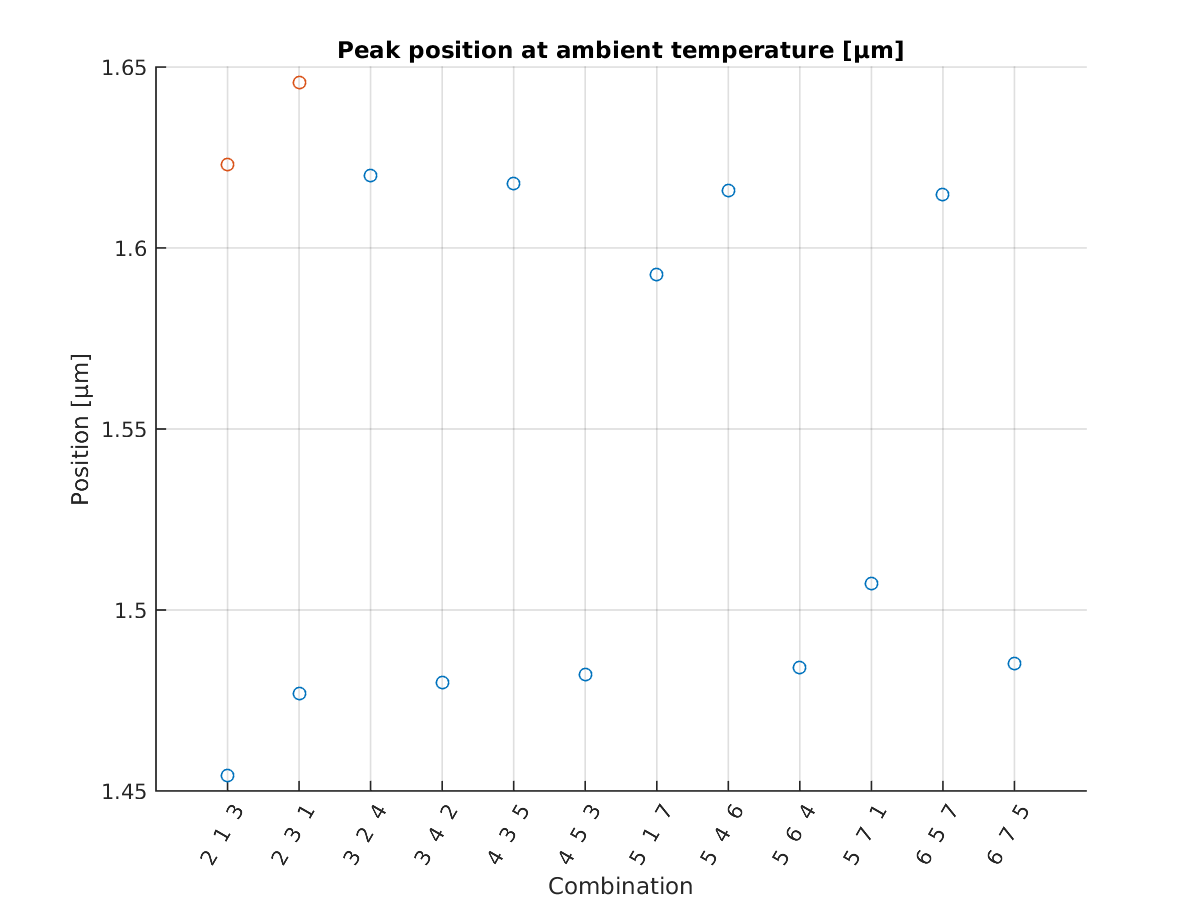
\includegraphics[width=.75\textwidth]{ppaat2.png}
	\caption{Peak position at $T_{amb}$. The label of the x axis are to be read as pump-signal-idler orders.}
	\label{fig_sym_pp@t2} 	% pp@t = bandwidth @ T_amb, 2 = no points at 1.55um
\end{figure}

\begin{figure}[!h]
	\centering
	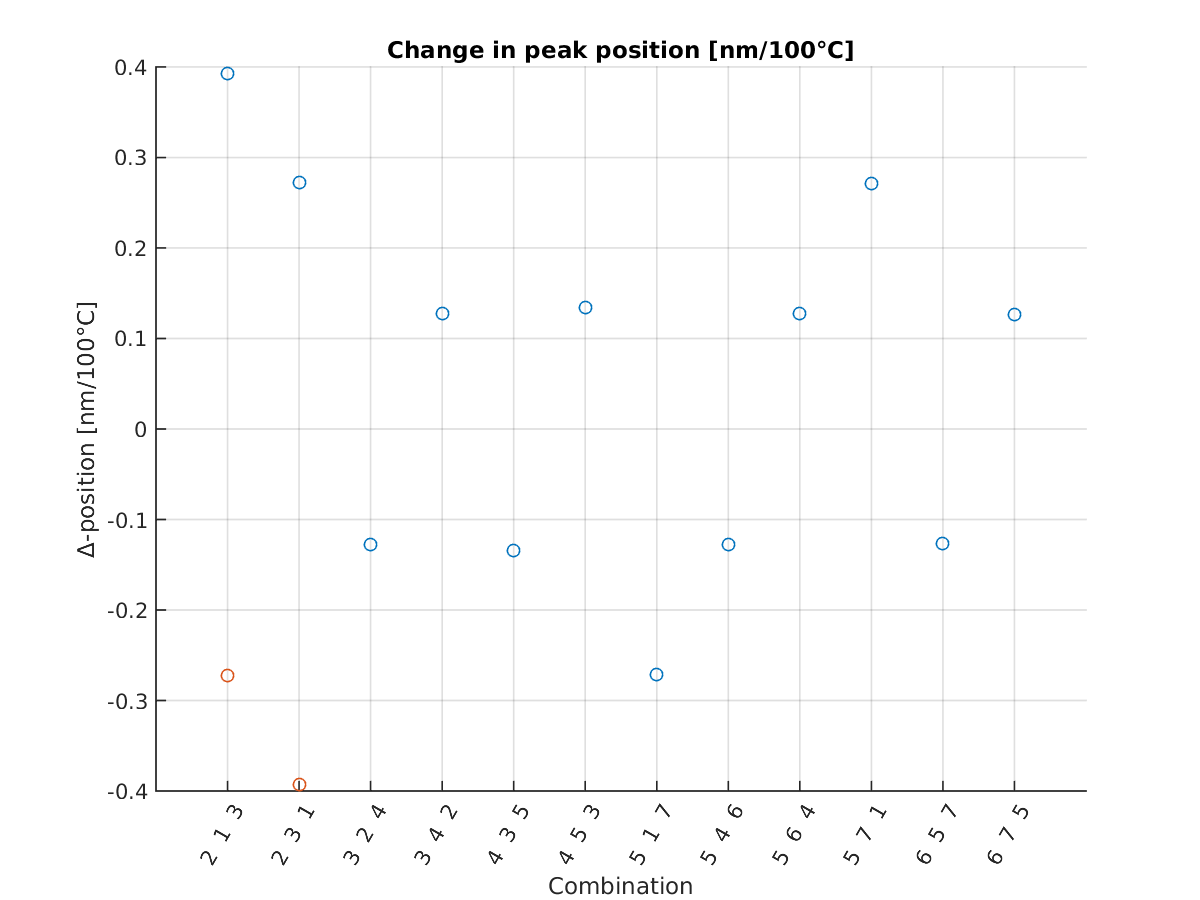
\includegraphics[width=.75\textwidth]{ppc2.png}
	\caption{Change of peak position.}
	\label{fig_sym_ppc2} % ppc = bandwidth change
\end{figure}

\begin{figure}[h!]
	\centering
	\begin{subfigure}[b]{0.75\textwidth}
		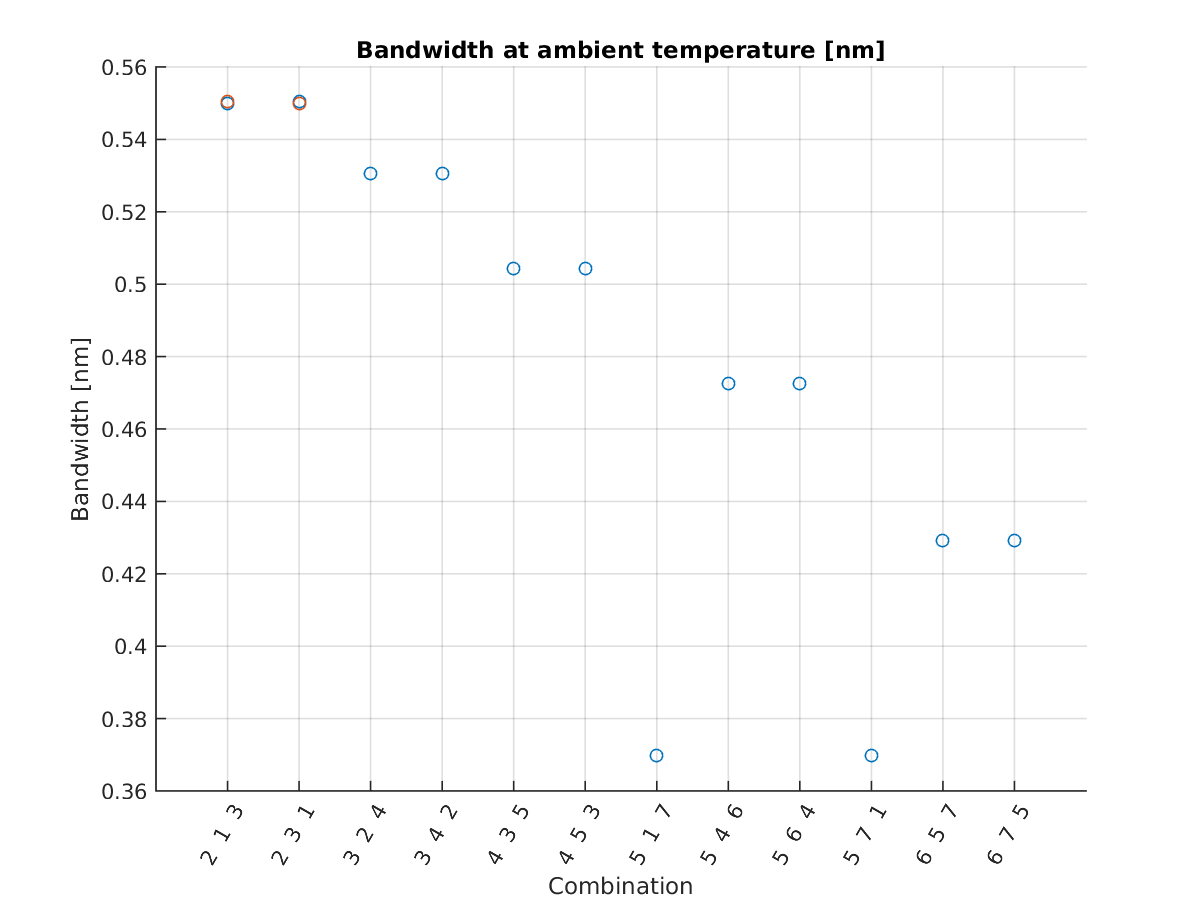
\includegraphics[width=1\textwidth]{baat2.png}
		\label{fig_sym_b@t2} % b@t = bandwidth @ T_amb
		\caption{Bandwidth at $T_{amb}$.}
	\end{subfigure}
	\begin{subfigure}[b]{0.75\textwidth}
		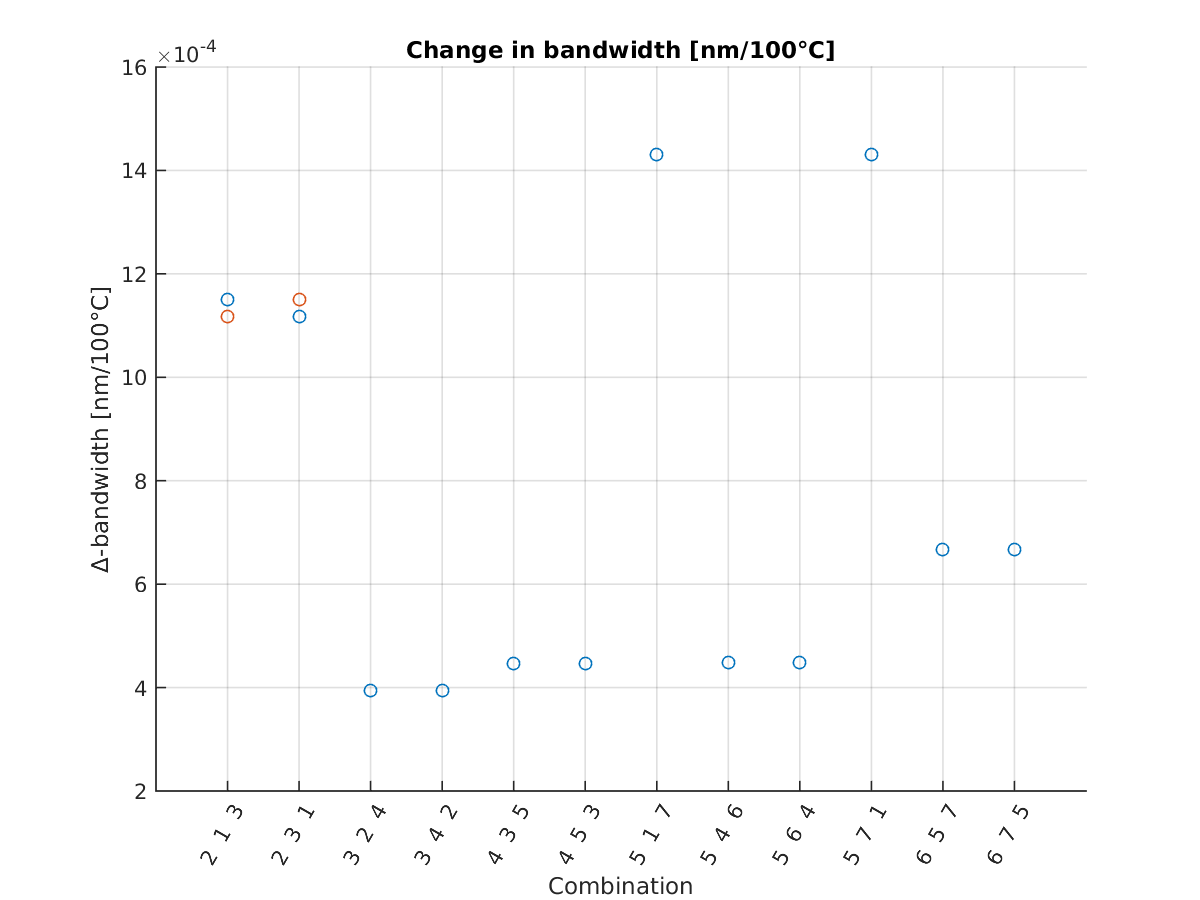
\includegraphics[width=1\textwidth]{bc2.png}
		\label{fig_sym_bc2} % bc = bandwidth change
		\caption{Change of bandwidth.}
	\end{subfigure}
	\caption{Bandwidth summary}
	\label{fig_sym_bw}
\end{figure}

\subsection{Second heater configuration}
In order to achieve a greater effect from the different temperature, we tried to move the heater from over the center of the core to the side.
This operation was intended to increase the difference of behaviour between low and high orders enabling thus the creation of new peaks in the coherence length.

The new geometry is represented in Figure (\ref{fig_geometry_asym}).
\begin{figure}[!ht]
	\centering
	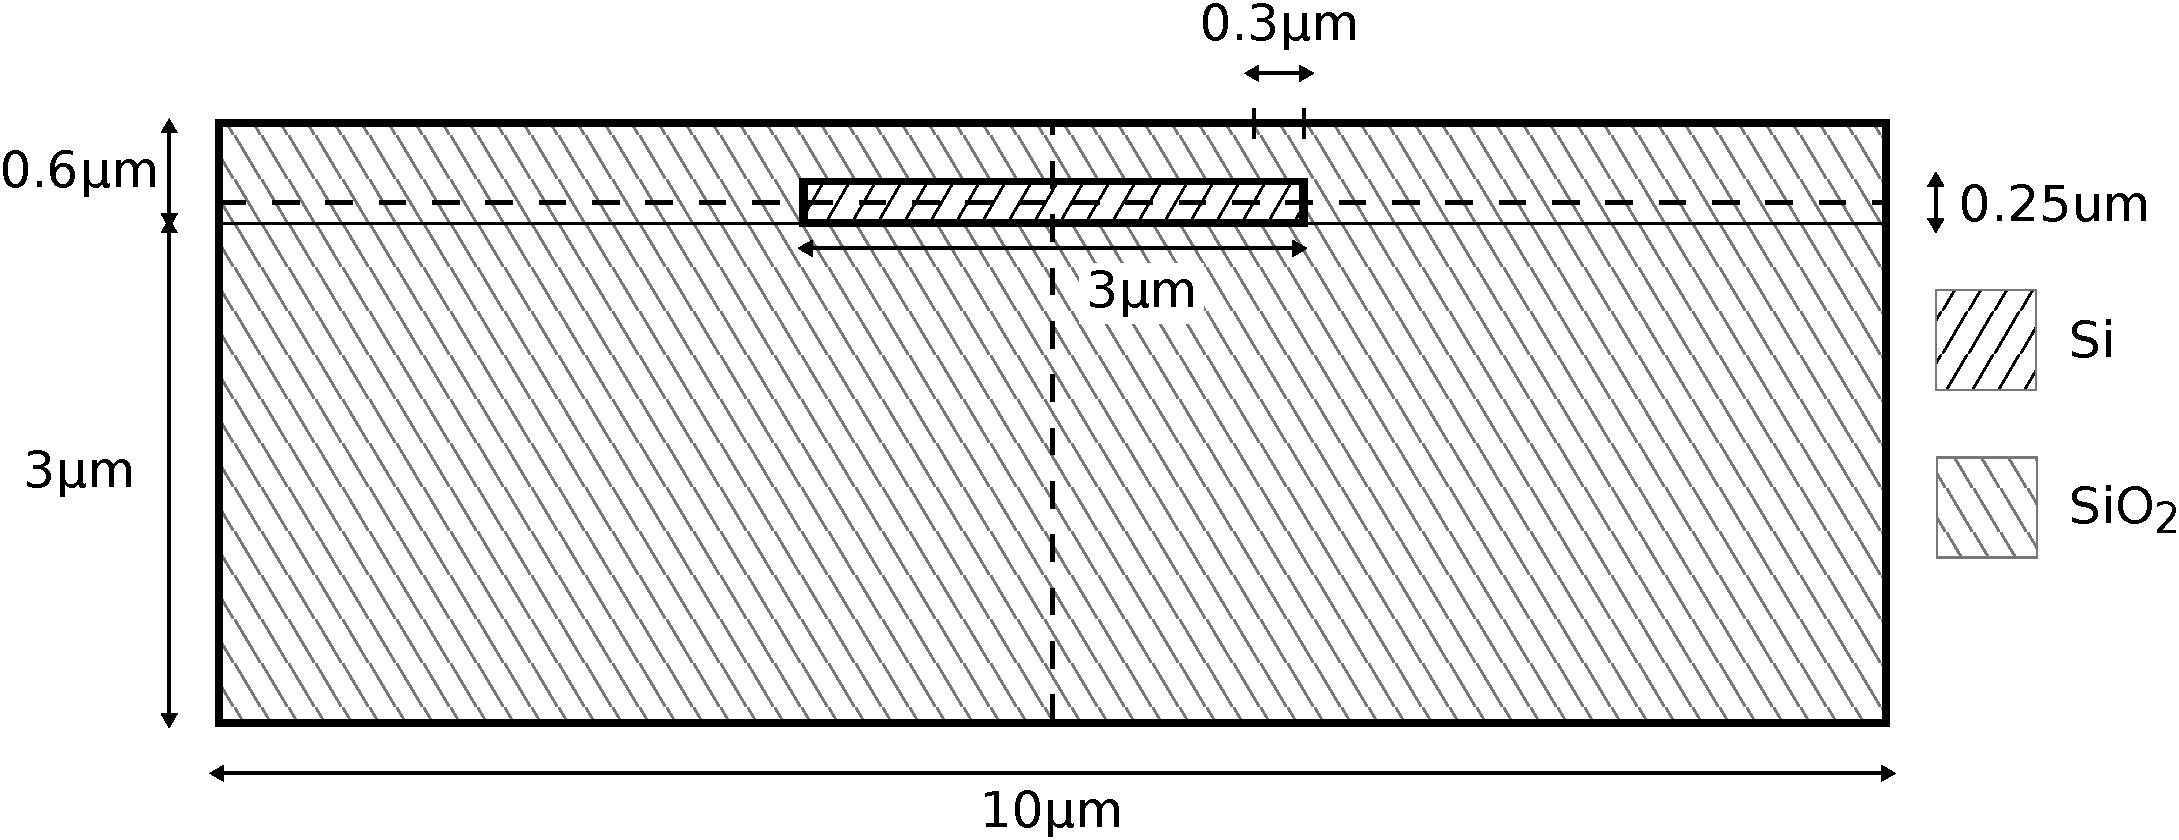
\includegraphics[width=1\textwidth]{geometryA.pdf}
	\caption{Scheme of the side heater configuration.}
	\label{fig_geometry_asym}
\end{figure}

\subsubsection{data aggregation}
Examining the graphs obtained from the data analysis of the asymmetric configuration, we noticed a variety of different situations.
Therefore we could not summarize the results with slopes and value at $T_{amb}$ anymore.


\section{Conclusions}
\subsection{Improvements}

There are a few improvements which were not introduced in our study because of the limited time available.
They could be eventually implemented in an extended study of this topic.

A rough list of them is proposed next:
\begin{itemize}
\item	The heater should be simulated as a metal conductor media, instead of a simple boundary condition, in addition to its thermal reservoir property. This is necessary because a metal plaque over the waveguide core could interfere with the wave propagation in the waveguide itself, drawing energy from the EM wave.

\item	Thermal expansion of materials should be considered.
While the thermal expansion coefficients of both silicon and silica are small, the temperature change is quite high.
It should not be lightly considered as a negligible contribution as it could change the waveguide geometry and therefore the modes.

\item	The aim of this study was limited to understanding if it was possible at all to control FWM with temperature.
It is also important to develop the correlation between temperature and efficiency of energy conversion from the pump to the idler.

\item	As next step in enhancing the influence of temperature on effective index, different core geometries could be studied.
This could greatly condition the wave propagation, but it is also a difficult problem with many degrees of freedom.

\end{itemize}

\subsection{Summary}

\cleardoublepage
\begin{thebibliography}{9}
\bibitem{agrawal} G. Agrawal. Nonlinear Fiber Optics, 5th edition. 2013
\bibitem{saleh} B. E. A. Saleh, M. C. Teich. Fundamentals of photonics, 2nd edition. 2007
\bibitem{n_db} http://refractiveindex.info/
\bibitem{spectrum} Lau, Ryan KW, et al. "Continuous-wave mid-infrared frequency conversion in silicon nanowaveguides." Optics letters 36.7 (2011): 1263-1265.
\end{thebibliography}
\end{document}
% Ref. \cite{agrawal}